\documentclass[UTF8]{ctexart}

\usepackage{tikz,esvect}
\usetikzlibrary{3d,calc,shapes}
\usepackage{graphicx}
\usepackage{subfigure}
\usepackage{varwidth}
\usepackage{scalefnt}

\pagestyle{empty} %% 无页眉页脚
\def\layersep{2.5cm}

\title{基础模型学习笔记}
\author{Wulnut}
\date{\today}

\begin{document}
    \maketitle
    \newpage
    \tableofcontents
    \newpage

    \section{元胞自动机}
    \subsection{概述}
    元胞自动机(cellular automata,CA) 是一种时间、空间、状态都离散,空间相互作用和时间因果关系为局部的网格动力学
模型,具有模拟复杂系统时空演化过程的能力。元胞自动机是一个空间和状态都是离散的模型。该模型可以用一个四元组表示:
    \begin{equation}
    C=(L_a, S, N_n, f)
    \end{equation}

    其中:
    \begin{itemize}
        \item $S$表示细胞状态,是一个有限的、离散的状态集合;
        \item $L_a$表示元胞空间,$a$是一个整数,表示细胞空间的维数;
        \item $N$表示领域内元素的组合,$n$表示邻居的个数
        \item $f$表示状态转移函数,即状态转移规则
    \end{itemize}

    \subsubsection{邻元}
    对于一个元胞,在空间位置上与它相邻的元胞称为它的\textbf{邻元}(有时也称作邻居),邻域和邻元的定义可以是多样的。

    \begin{figure}[h]
        \centering
        \includegraphics[width=8cm]{img/CA_table.png}%%latex不支持中文路径
        \caption{一维CA网格}

        \includegraphics[width=8cm]{img/CA_table(1).png}
        \caption{二维CA网格}
    \end{figure}

    \newpage
    每个元胞有若干个状态,如:
    \begin{itemize}
        \item 物理系统:(分子)固态,液态
        \item 生物系统:(细胞)死or活
        \item 社会系统: (个人)相信与不相信谎言
        \item 政治系统: (国家)战争与妥协\ldots
    \end{itemize}

    
    在各种CA模型中,每个等份(单元格)代表一个元胞,CA的网格可以有不同的形式(维数,大小):
    \begin{itemize}
        \item 一维的CA模型是将直线分成若干相同的等份
        \item 二维的CA模型是将一个平面分成许多正方形、六边形或三角行的网格(最常见的是将其划分成正方形);
        \item 三位的CA模型将空间划分成许多立体网格。
    \end{itemize}
    
    \begin{figure}[h]
        \centering
        \includegraphics[width=8cm]{img/CA_model.png}
        \caption{一维CA模型}
        \includegraphics[width=8cm]{img/CA_model(1).png}
        \caption{二维CA模型}
    \end{figure}

    \subsection{规则}
    根据每个元胞及邻元的不同状态,由于状态更新规则决定这个元胞下一个时刻的状态,序号$i$个体在$t=1$,\dots,$n$时刻的状态:
    \begin{equation}
        S_t^{t+1}=f(S_i^t,N^t)=f(S_i^t,S_1^t,S_2^t,..,S_n^t)
    \end{equation}

    其中$S_i^t,S_1^t,S_2^t,\dots,S_n^t$为个体$i$的邻元在$t$时刻的状态。


    规则可以是确定型的,也可以是随机型的。对于一个一维的CA,一个细胞具有两种可能的状态如生or死,相信或者不相信等等,表示为0 or 1。


    如果规则一:我使用下图的左边的邻元定义
    定义其状态更新规则:当一个个体的两个邻元都活或都死,该个体在下一时刻为死;反之,他的状态在下一时刻变为活。

    \begin{figure}[h]
        \centering
        \includegraphics[width=12cm]{img/rule_table.png}
        \caption{规则表(1)}
    \end{figure}

    再如规则二:我仍然使用当前左边邻元定义,但重新定义其状态
    更新规则为:当个体的两个邻元都活或都死,该个体再下一时刻\textbf{改变状态};反之,\textbf{该个体的状态在下一时刻保持不变}。

    \begin{figure}[htb]
        \centering
        \includegraphics[width=12cm]{img/rule_table(1).png}
        \caption{规则表(2)}
        
    \end{figure}

    \subsection{构建模型}

    考虑如下问题:
    \begin{itemize}
        \item 确定系统中有那些个体,如何分类?
        \item 个体有几种状态,分别是什么;
        \item 个体所处空间形式,是一位,二维还是多为;
        \item 个体的邻元形式及个数,这与网格形式及交互群体规模有关
        \item 根据个体状态、网格形式及邻元,确定个体状态的演变规则。        
    \end{itemize}

    \vspace{0.5cm}
    \textbf{此外还需要,确定:}
    \begin{itemize}
        \item 系统中的个体与单元格是否一致。
    \end{itemize}
    简单的、经典的CA模型中,单元格与个体不加区分,每个单位格就是一个个体,个体始终在单元格中,个体的状态即为单元格的状态。但在一些
    复杂系统中,尤其在个体可以移动的系统中,将个体与单元格区分更为方便。

    \begin{itemize}
        \item 系统中是否离散事件。
    \end{itemize}
    采用CA模型描述的系统,每个时刻都需根据规则确定元胞的状态。除此之外,有的系统中某些个体会在特定时刻(有条件或无条件)发生状态变
    化,此时可以采用离散时间仿真方法,将该时刻列入事件表,根据事件表处理该类事件。
    
        \vspace{0.5cm}
        \begin{figure}[htb]
            \scalefont{0.5}%% pgf / tikz创建图表用来控制字体大小
            \centering
        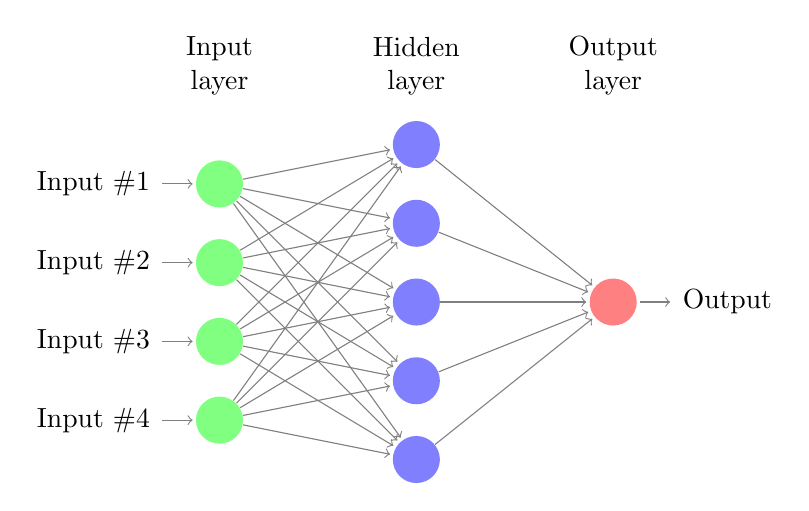
\begin{tikzpicture}[shorten >=1pt,->,draw=black!50, node distance=\layersep]
            \tikzstyle{every pin edge}=[<-,shorten <=1pt]
            \tikzstyle{neuron}=[circle,fill=black!25,minimum size=17pt,inner sep=0pt]
            \tikzstyle{input neuron}=[neuron, fill=green!50];
            \tikzstyle{output neuron}=[neuron, fill=red!50];
            \tikzstyle{hidden neuron}=[neuron, fill=blue!50];
            \tikzstyle{annot} = [text width=4em, text centered]
        
            % Draw the input layer nodes
            \foreach \name / \y in {1,...,4}
            % This is the same as writing \foreach \name / \y in {1/1,2/2,3/3,4/4}
                \node[input neuron, pin=left:Input \#\y] (I-\name) at (0,-\y) {};
        
            % Draw the hidden layer nodes
            \foreach \name / \y in {1,...,5}
                \path[yshift=0.5cm]
                    node[hidden neuron] (H-\name) at (\layersep,-\y cm) {};
        
            % Draw the output layer node
            \node[output neuron,pin={[pin edge={->}]right:Output}, right of=H-3] (O) {};
        
            % Connect every node in the input layer with every node in the
            % hidden layer.
            \foreach \source in {1,...,4}
                \foreach \dest in {1,...,5}
                    \path (I-\source) edge (H-\dest);
        
            % Connect every node in the hidden layer with the output layer
            \foreach \source in {1,...,5}
                \path (H-\source) edge (O);
        
            % Annotate the layers
            \node[annot,above of=H-1, node distance=1cm] (hl) {Hidden layer};
            \node[annot,left of=hl] {Input layer};
            \node[annot,right of=hl] {Output layer};
        \end{tikzpicture}
        \caption{nice}
        \end{figure}
        

    












    \newpage
    \section{主成分分析}
    \newpage

    \section{聚类分析}

\end{document}